%chapter{Background Information}
%Fountain Codes
%Systematic Raptor Codes

\hspace{\parindent} The goal of this chapter is to briefly review some major concepts which have been used in this thesis. The following section introduces the FEC over time varying and an unknown erasure channel which is considered as the model of the channel under study. Next, we discuss the properties, encoding and decoding scheme of raptor FEC codes.
  

\section{Forward Error Correction and Erasure Channel}
A FEC code as described in \cite {griesser2009forward} is a scheme that controls error/losses in the data transmission. The sender encodes the message in a redundant way by using an error-correcting code \cite{macwilliams1977theory} \cite{peterson1972error}, this redundancy allows the receiver to detect a limited number of errors that may occur anywhere in the message, and correct these errors without feedback with the sender. 
\par
An erasure channel is a communication channel model where a transmitter sends a bit (a zero or a one), and the receiver either receives the bit or it receives a message that the bit was not received ("erased").Though this channel was more of a theoretical concept when it was introduced, it is a perfect model in many existing and emerging communication systems.
\begin{figure}[htbp]
\begin{center}
\mbox{
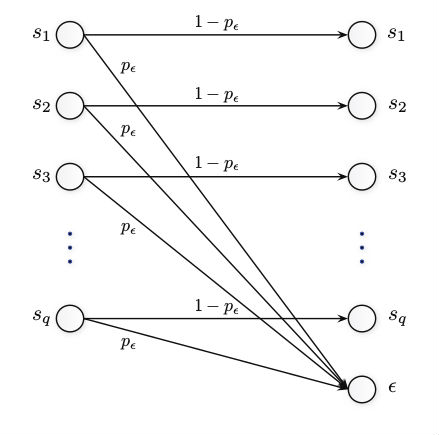
\includegraphics[width=3.5in]{Figures/erasure1}}
\caption{A \textit{q}-ary erasure channel with an input alphabet of size q, and a output alphabet of size \textit{q}+ 1.}
\label{erasure_channel}
\end{center}
\end{figure}

Probably the most practical erasure channel is a link in a packet network such as the Internet. The packets transmitted on these links are either received without error or not received. More generally, any noisy channel protected with an error-correcting code behaves like an erasure channel since the received symbol is either decoded or completely useless.
% If a symbol is received completely, the error correcting code recovers the transmitted symbol perfectly, \todo {Redundant }and the transmission can be supposed to be performed noiseless. Else if, the received symbol is incomplete and not decodable then this can be taken as an erasure.
\par
The model of a \textit{q}-ary erasure channel could be described as in figure ~\ref{erasure_channel}. The set of input symbols of such channel is \{s\textsubscript{1}, s\textsubscript{2}, . . , s\textsubscript{\textit{q}}\}, while output set consists of all possible inputs and an erasure $\epsilon$. Each input symbol is assumed to have a 1$-$\textit{p\textsubscript{$\epsilon$}} probability of successful transmission, and will be erased by channel with probability \textit{p\textsubscript{$\epsilon$}}. 

Raptor codes can be defined as a symbols belonging to an alphabet \textit{q}, and define multiplication and addition over the set of this alphabets. As an obvious choice for the symbol\textquotesingle s  alphabet is then a Galois field of size \textit{q} which is referred as \textit{GF(q)}. The coefficients for the random linear combinations will also be selected from the same alphabet.



\section{Fountain Codes}
Fountain codes, also known as \enquote{\textit{rateless}} codes or \enquote{\textit{Digital Fountain}} are class of erasure codes with the property to generate a theoretically endless stream of output symbols \cite{blahut1983theory} \cite{lin2004error}. Where each symbol provides partial information about the original symbols, since each output symbol is a random linear combination of the original message symbols. Once the receiver receives required amount of symbols, its starts to recover the original information. Figure \ref{fountain} shows encoding of fountain codes briefly and following is the terminology:\\
\textbf{Symbol}\\
A symbol is defined as a smallest unit of data. These units are measured in bytes, also known as the symbol size. Each gray color box represents a symbol in fig \ref{fountain}\\
\begin{figure}[h!]
\begin{center}
\mbox{
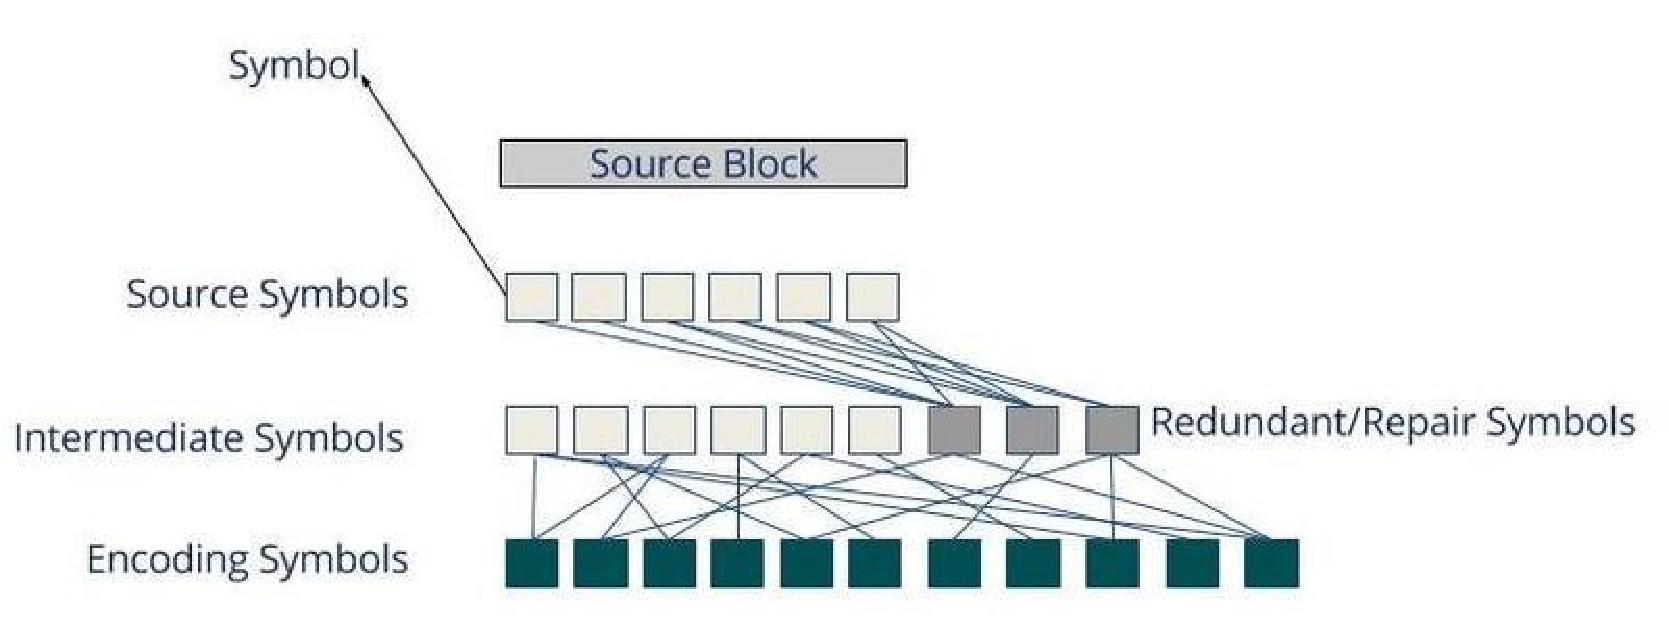
\includegraphics[width=5.8in]{Figures/fountain}}
\caption{Fountain codes terminology}
\label{fountain}
\end{center}
\end{figure}

\noindent
\textbf{Source symbols} \\
The smallest unit of data used during the encoding process. All source symbols within a source block have the same size. \\

\noindent
\textbf{Source Block}\\
A block of source symbols that are considered together for Raptor encoding purposes.\\
\textbf{Redundant/Repair symbols}\\
Redundant symbols are generated from a source block and have the same size as the source symbols of that source block.\\
\textbf{Intermediate symbols}\\
Symbols generated from the source symbols using an inverse encoding process. The repair symbols are then generated directly from the intermediate symbols. The intermediate symbols are not included in data packets.\\
\textbf{Encoding symbols}\\
A symbol that is included in a data packet.  The encoding symbols consist of the source symbols and the redundant symbols.
\section{Raptor Forward Error Correction Code}
Raptor Code is called either the Raptor 10 code or the R10 code. This is a class of fountain code that has the capability of Forward Error Correction (FEC). R10 is a also fully-specified FEC scheme, that is, independent implementors can implement both the encoder and the decoder from a specification that is an Internet Engineering Task Force (IETF) Request For Comments (RFC). 

Raptor codes can be realized in two ways: the non-systematic and the systematic raptor codes. The method used in encoding process is notable difference between the two kinds. The properties of raptor codes include linear time encoding \cite{luby2006raptor} (independent of the quantity of repair symbols generated) and linear time decoding (independent to amount of loss), ideal performance under any channel loss conditions, and ability to support large file size.

Raptor Codes used in this research are systematic codes, that are, redundant data can simply be appended to the original symbols, and receivers do not need to recover the original symbols if received correctly. Raptor code is designed to support a number of original symbols \textit{K} between 4 to 8192. This section gives a detail construction of R10 code. We make references to the specification of this code from RFC 5053 \cite{luby2007rfc} and use the same terminology.

\subsection{Overview}
Raptor codes as shown in fig \ref{overview} are a concatenation of a pre-code and LT code \cite{khisti2003tornado}, with pre-code usually being Low Density Parity Check (LDPC) \cite{gallager1962low} code, defined over Galois field with 2 elements \textit{GF(2)}. This pre-code maps \textit{K} original symbols (or for a group of original symbols) onto L intermediate symbols (L $>$ K). In the next step, each encoded symbol is formed by performing an exclusive-or (XOR) operation on randomly selected subsets of symbols, chosen from L intermediate symbols, based on degree distribution as specified in section 5.4.4.2 in \cite{luby2007rfc}. The operation of generating encoded symbols constitutes the LT code which is responsible for the rateless property of Raptor codes -- that is the ability to generate as many symbols as needed on-the-fly.
\\
\begin{figure}[htbp]
\begin{center}
\mbox{
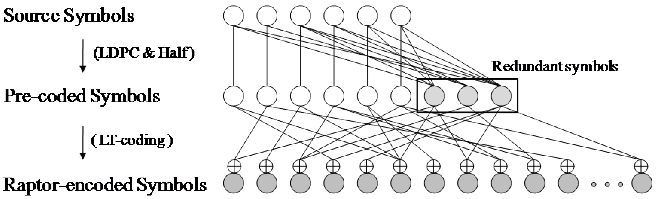
\includegraphics[width=5.2in]{Figures/overview}}
\caption{Two encoding steps of Raptor codes, LT and LDPC \cite{ha2017block}}
\label{overview}
\end{center}
\end{figure}
\par
Section ~\ref{encoder} describes the systematic Raptor code encoder. A number of possible decoding algorithms are possible. The efficient decoding algorithm used for this thesis simulations is described in section~\ref{decoder}.

\subsection{Encoder} \label{encoder}

The encoding process is summarized in two main blocks, namely \textit{Code Constraint Processor} and \textit{LT Encoder}. They both are represented by their equivalent generator matrices. A block diagram of Systematic Raptor Encoder/Decoder is shown in figure~\ref{Raptor_en_dc}.

\subsubsection{Code Constraint Processor}
\label{CCP}
Let \textbf{t} denote \textit{K} (4 $<$ \textit{K} $<$ 8192) original symbols that are to be encoded. The \textbf{d} that is given as input to Raptor encoder, contains \textit{L = K + H + S} symbols. Where S is the number of Low Density Parity Check (LDPC) redundant symbols and H is the High Density Parity Check (or) half symbols. These symbols depend on large number of original symbols, defined over GF(2) as:
\begin{equation}
\textbf{d}_{[0:L-1]} = [\textbf{z}^{T} \ \textbf{t}^{T}]^{T}
\end{equation}
where \textbf{z}\textsubscript{[0:H\thinspace+\thinspace S\thinspace \textminus 1]} is a vector of zeros. The parameter \textit{S} is the smallest prime number such that
\begin{equation}
S \geq \lceil{0.01 \times K }\rceil + X 
\end{equation}
where X is smallest positive integer such that 
\begin{equation}
X(X-1) \geq 2K
\end{equation}
Similarly, \textit{H} is the smallest integer such that 
\begin{equation}
\begin{pmatrix}
           H \\
          \lceil H/2 \rceil
\end{pmatrix}
=
\frac{H!}{2(H/2)!}
\geq K + S
\end{equation}
\textit{H} is chosen like this so that the columns of the matrix G\textsubscript{\textit{Half}} in matrix of equation~\ref{eq:matrix} are all distinct.
\par
Intermediate symbols, \textbf{c} are generated when \textbf{d} multiplies with the inverse of the pre-coding matrix \textbf{A} as:
\begin{equation}
c_{[0:L-1]} = A_{L \times L}^{-1} {\,\cdot\,} \textbf{d}_{[0:L-1]} 
\end{equation}
with 
\begin{equation}\label{eq:matrix}
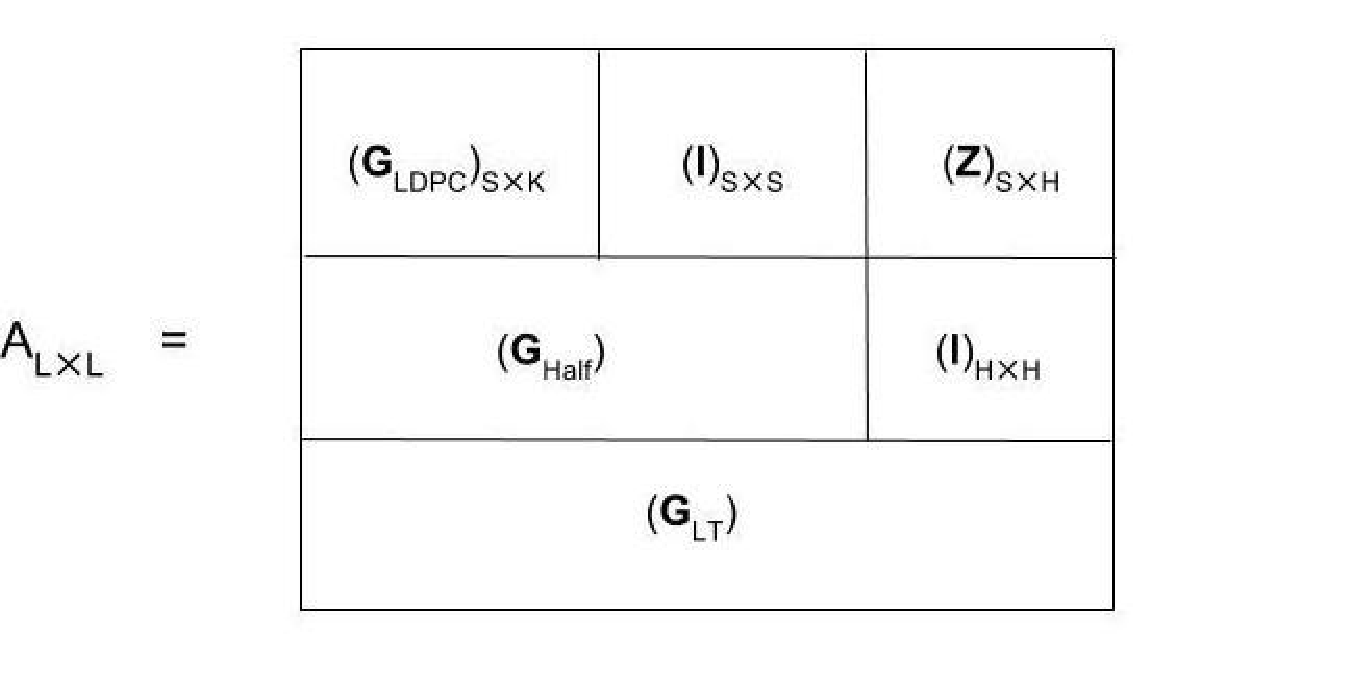
\includegraphics[width=3.8in]{Figures/matrix}
\end{equation}
where submatrices \textbf{I}\textsubscript{\textit{S}} and \textbf{I}\textsubscript{\textit{H}} are identity matrices, and \textbf{Z} is a zero sub-matrix with dimension \textit{S} $\times$ \textit{H}; \textbf{G}\textsubscript{\textit{LDPC}} is a \textit{S} $\times$ \textit{K} low density parity check (LDPC) generator sub-matrix and is defined as follows:
\begin{equation}
G_{\textit{LDPC}}{\,\cdot\,}[c[0], . . . ,c[K-1]]^{T} =  (c[K], . . . ,c[K+S-1])^{T}
\end{equation}
G\textsubscript{\textit{Half}} is a  \textit{H} $\times$ (\textit{K + S}) generator sub-matrix of the Half/HDPC symbols, defined as:
\begin{equation}
G_{\textit{Half}}{\,\cdot\,}[c[K + S - 1], . . . ,c[K - 1]]^{T} =  [c[K + S], . . . ,c[K + S + H - 1]]^{T}
\end{equation}
G\textsubscript{\textit{LT}} is a \textit{K} $\times$ \textit{L} generator sub-matrix in \textbf{A} for the first \textit{K} symbols that contributes a Raptor codes systematic:
\begin{equation}
G_{\textit{LT}}{\,\cdot\,}[c[0], . . . ,c[L - 1]]^{T} =  [t[0], . . . ,t[K - 1]]^{T}
\end{equation}

\begin{figure}[htbp]
\begin{center}
\mbox{
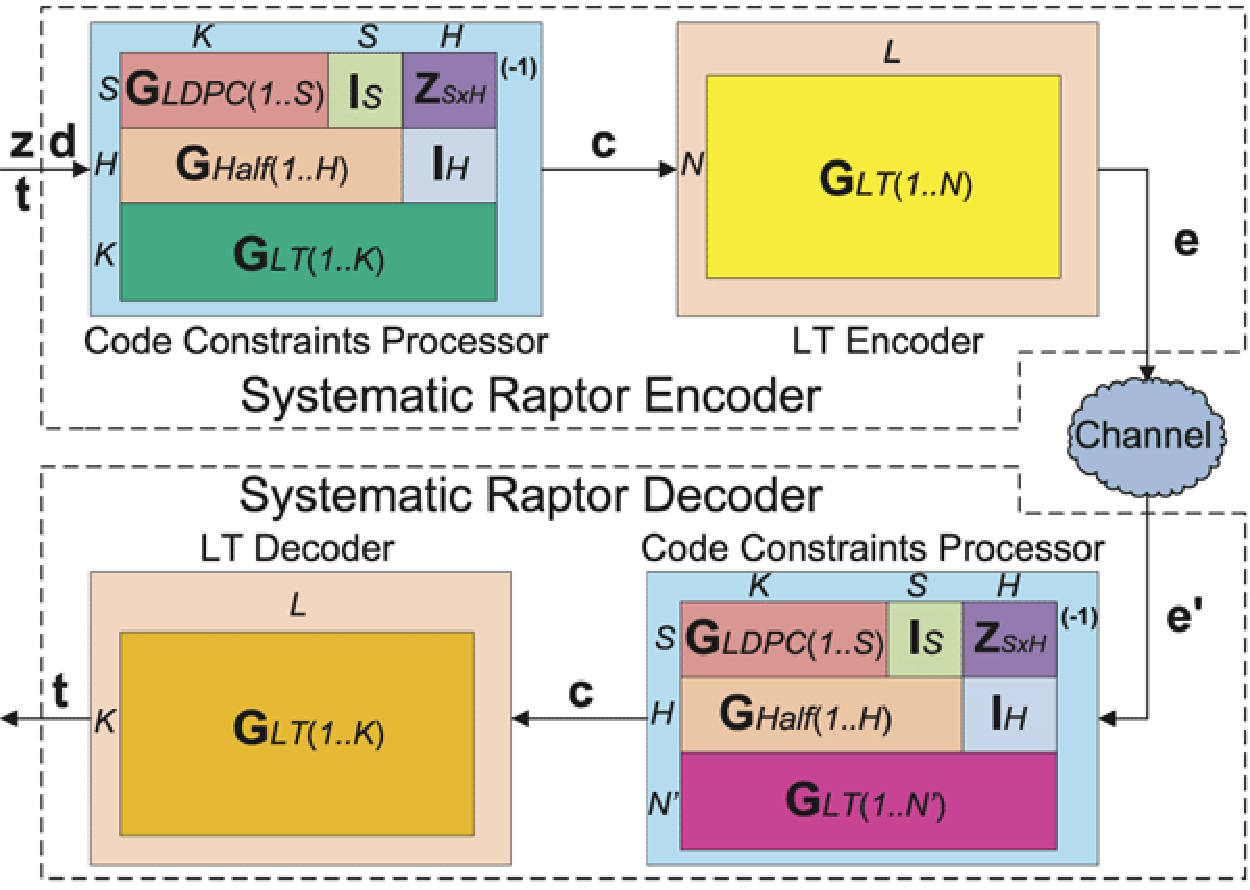
\includegraphics[width=5.5in]{Figures/encoder}}
\caption{Block diagram of Raptor Encoder/Decoder \cite{mladenov2011implementation}}
\label{Raptor_en_dc}
\end{center}
\end{figure}

\subsubsection{LT Encoder}
\label{lt}
The source vector \textbf{t} is pre-processed by the intermediate symbols generator, then the LT encoder generate any number of encoded symbols \textbf{e} according to:
\begin{equation}
G_{LT}{\,\cdot\,}c = \textbf{e}_{[0:N - 1]}
\end{equation}
where G\textsubscript{\textit{LT}} is an  \textit{N} $\times$ \textit{L} LT generator matrix, with \textit{N} $\geq$ \textit{K}. The value \textit{N} is selected to be sufficiently larger than \textit{K} to compensate for the possible loss of encoded symbols during transmission and thus to make matrix \textbf{A} invertible at the decoder side. 
\begin{equation}
e[i] = d[H + S + i], \forall_{i=0,...,K - 1}
\end{equation}
This is because G\textsubscript{\textit{LT}} for symbols 0,..., \textit{K $-$ 1} is included in the pre-processing matrix \textbf{A}, making Raptor code systematic. 
\par
For a fixed value of \textit{K}, submatrices \textbf{G}\textsubscript{\textit{LDPC}}, \textbf{G}\textsubscript{\textit{Half}}, \textbf{G}\textsubscript{\textit{LT}}(0, . . ., \textit{K $-$ 1}) are pre-generated once and stored in the memory of the sender. The structure of G\textsubscript{\textit{LT}} matrix shows how the encoded output symbols \textbf{e} are generated from the intermediate symbols \textbf{c}. The \enquote{1} values on the g\textsuperscript{th} row of matrix \textbf{G}\textsubscript{\textit{LT}} identify the intermediate symbols that are XORed to generate encoded symbol e[g].
\par
Before the encoded symbols are transmitted, they are grouped and augmented with an Encoding Symbol Identifier (ESI). Encoded symbols with ESIs 0, . . . , \textit{K $-$ 1} corresponds to source symbols and the ESIs \textit{K, K + 1}. . . corresponds to redundant (or) repair symbols. This is advantageous, as these ESIs help the decoder to distinguish the original symbols and the redundant symbols while decoding; the details which are omitted from the diagram for simplicity. 

\subsection{Decoder} \label{decoder} 
The Raptor decoder exchanges the position of \textit{Code Constraint Processor} and \textit{LT Encoder}, more precisely \textit{LT Decoder}, as illustrated in the figure~\ref{Raptor_en_dc}. The input vector \textbf{e}\textquotesingle \: containing \textit{N}\textquotesingle \: \textit{(K $\leq$ N\textquotesingle \: $\leq$ N)} encoded symbols (may not be in order) is padded with \textit{S + H} zeroes to size it to \textit{(M = N\textquotesingle + S + H)}. Starting with \textit{N\textquotesingle \:= K} the value of \textit{N\textquotesingle} is iteratively incremented to make the matrix \textbf{A} invertible. The difference \textit{(N\textquotesingle \:$-$ K)} is equal to or greater than the number of received encoded symbols lost in the channel. 
\par
The decoding is performed according to:
\begin{equation}
\label{decode_equ_1}
c_{[0:L-1]} =  [\textbf{z}^{T} \, \textbf{e\textquotesingle}^{T}] {\,\cdot\,} A_{M \times L}^{-1}
\end{equation}

\begin{equation}
t_{0:K-1} = \textbf{G}_{LT} {\,\cdot\,} \textbf{c}_{[0: L-1]}
\label{decode_equ_2}
\end{equation}
where \textbf{G}\textsubscript{\textit{LT}} is a\textit{ K $\times$ L} LT generator matrix.
\par
At the decoder side the sub-matrix \textbf{G}\textsubscript{\textit{LT}}(1..\textit{N\textquotesingle}) is first built from the input data. The ESI of the n\textsuperscript{th} received encoded symbol is used to generate the n\textsuperscript{th} row of the sub-matrix \textbf{G}\textsubscript{\textit{LT}}(1..\textit{N\textquotesingle}) through the LT encoding process.
\par
Decoding a source block is equivalent to decode c\textsubscript{[0:L$-$1]} from known matrix \textbf{A} and vector \textbf{e\textquotesingle}. It is clear from equation ~\ref{decode_equ_1} that c\textsubscript{[0:L$-$1]} can be decoded if and only if the rank of matrix \textbf{A\textsuperscript{-1}} over \textit{GF(2)} is L. Once c\textsubscript{[0:L$-$1]} is decoded, the source symbols can be recovered. `\ref{decode_equ_2}.
\par
The decoding algorithm of Raptor code uses Gaussian Elimination (GE) (using row operations and row and column reordering) to transform \textbf{A} to L $\times$ L identity matrix after  discarding M $-$ L rows.
\par
The transformation process is summarized below into four phases and is shown in figure ~\ref{decoder_fig}

% Add decoder image
\begin{figure}[htbp]
\begin{center}
\mbox{
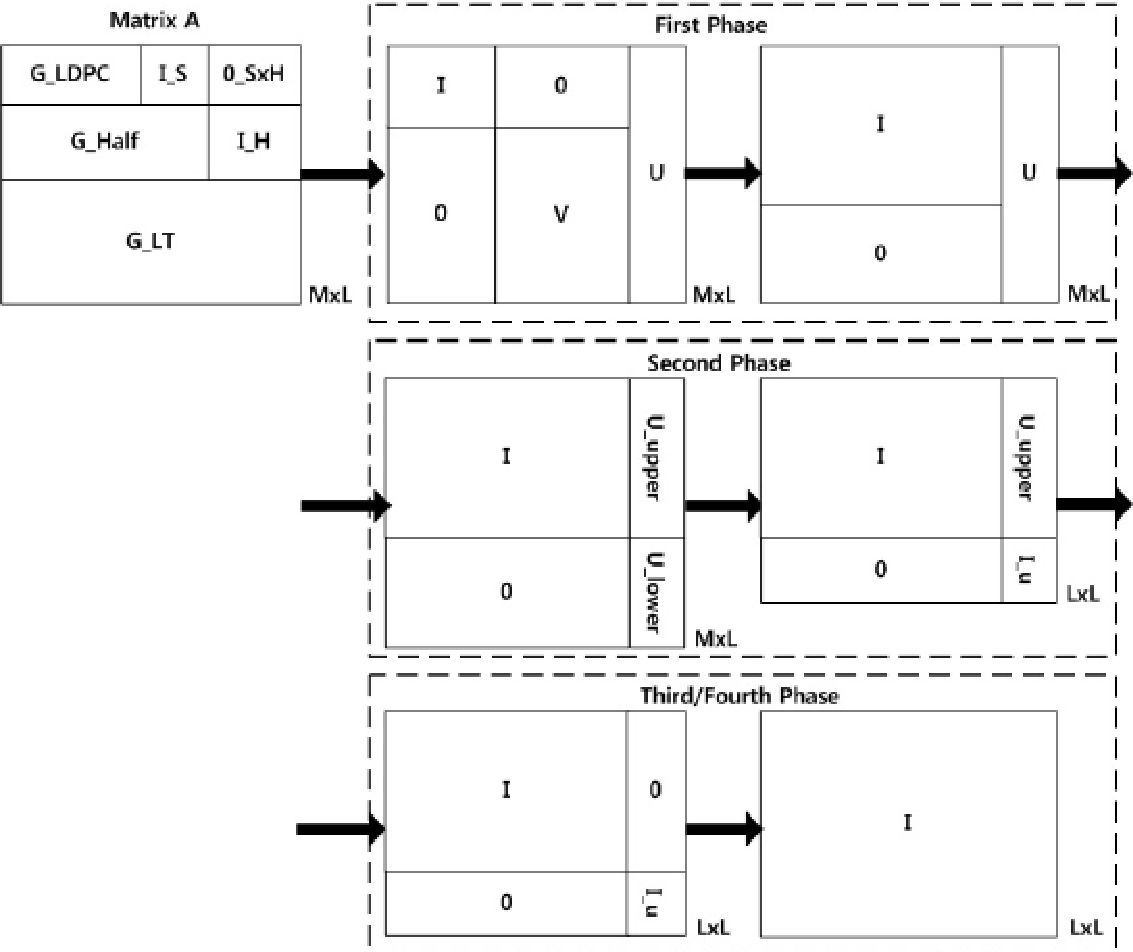
\includegraphics[width=5.5in]{Figures/decoder}}
\caption{Illustration of four phases to transform matrix A into an identity matrix \cite{wu2013fast}}
\label{decoder_fig}
\end{center}
\end{figure}

In the first phase, the matrix \textbf{A} is converted to three sub-matrices: I, Zero sub-matrix, and U as shown in Figure. In this figure, V is an intermediate matrix. In the beginning of phase one, V = A and I and U are Null matrices. 
\par 
For each iteration, a row of V, with the minimum non-zero degree r, is chosen, where the degree of a row is defined as the number of elements \enquote{1} it has. Then, the chosen row is exchanged with the first row in V. All the columns of V are reordered so that the first and the last r $\-$ 1 elements of the first row are \enquote{1}. Then, the other rows which have ones in their first column are XORed with the first row so that their columns become \enquote{0}. The rank of sub-matrix \textbf{I} is increased by 1 and the number of columns in U is increased by r$\-$1. This process is repeated until the sum of columns of I and U is equal to L. This decoding phase fails when no non-zero row remains in V before V disappears, that is, the sum of columns of I and U is less than L and elements in all rows of V are zero.
\par
In the second phase, the sub-matrix U is partitioned into U\textsubscript{\textit{upper}} and U\textsubscript{\textit{lower}}, where U\textsubscript{\textit{upper}} consists of the first i rows and U\textsubscript{\textit{lower}} contains the remaining M $-$ i rows. If the rank of U\textsubscript{\textit{lower}} is less than u, the decoding of second phase fails. Otherwise, GE is performed on U\textsubscript{\textit{lower}} to transform it into an identity matrix with rank u. Then, the last M $-$ L rows of A\textsubscript{M $\times$ L} are discarded.
\par
In the third phase, a pre-computation matrix U\textquotesingle \: with ceil(u/8) $\times$ 255 rows and u columns, is generated based on I\textsubscript{u}.
\par
In the fourth phase, the matrix U\textquotesingle \: is used to zero out U\textsubscript{\textit{upper}} and thus converts A into the L $\times$ L identity matrix.
\par
Successful decoding depends on the transformation process discussed above. The intermediate symbols c\textsubscript{[0:L$-$1]} can be decoded in the meantime, based on the row operations and row/column exchanges occurring during the transformation process.

\section{Raptor Code applications and advancements}
Fountain Codes have been adopted by the Third Generation Partnership Project (3GPP), Digital Video Broadcasting (DVB), Internet Protocol Television (IPTV) and Internet Engineering task Force (IETF). According to the Digital Fountain, raptor and its most advanced code raptorQ \cite{rfc6330} code is claimed as one of the most advanced forward error correction code for data networks.





























